\documentclass{beamer}
\usepackage{amsmath}
\usepackage[english]{babel} %set language; note: after changing this, you need to delete all auxiliary files to recompile
\usepackage[utf8]{inputenc} %define file encoding; latin1 is the other often used option
\usepackage{csquotes} % provides context sensitive quotation facilities
\usepackage{graphicx} %allows for inserting figures
\usepackage{booktabs} % for table formatting without vertical lines
\usepackage{textcomp} % allow for example using the Euro sign with \texteuro
\usepackage{stackengine}
\usepackage{wasysym}
\usepackage{tikzsymbols}
\usepackage{textcomp}
\newcommand{\bubblethis}[2]{
        \tikz[remember picture,baseline]{\node[anchor=base,inner sep=0,outer sep=0]%
        (#1) {\underline{#1}};\node[overlay,cloud callout,callout relative pointer={(0.2cm,-0.7cm)},%
        aspect=2.5,fill=yellow!90] at ($(#1.north)+(-0.5cm,1.6cm)$) {#2};}%
    }%
\tikzset{face/.style={shape=circle,minimum size=4ex,shading=radial,outer sep=0pt,
        inner color=white!50!yellow,outer color= yellow!70!orange}}
%% Some commands to make the code easier
\newcommand{\emoticon}[1][]{%
  \node[face,#1] (emoticon) {};
  %% The eyes are fixed.
  \draw[fill=white] (-1ex,0ex) ..controls (-0.5ex,0.2ex)and(0.5ex,0.2ex)..
        (1ex,0.0ex) ..controls ( 1.5ex,1.5ex)and( 0.2ex,1.7ex)..
        (0ex,0.4ex) ..controls (-0.2ex,1.7ex)and(-1.5ex,1.5ex)..
        (-1ex,0ex)--cycle;}
\newcommand{\pupils}{
  %% standard pupils
  \fill[shift={(0.5ex,0.5ex)},rotate=80] 
       (0,0) ellipse (0.3ex and 0.15ex);
  \fill[shift={(-0.5ex,0.5ex)},rotate=100] 
       (0,0) ellipse (0.3ex and 0.15ex);}

\newcommand{\emoticonname}[1]{
  \node[below=1ex of emoticon,font=\footnotesize,
        minimum width=4cm]{#1};}
\usepackage{scalerel}
\usetikzlibrary{positioning}
\usepackage{xcolor,amssymb}
\newcommand\dangersignb[1][2ex]{%
  \scaleto{\stackengine{0.3pt}{\scalebox{1.1}[.9]{%
  \color{red}$\blacktriangle$}}{\tiny\bfseries !}{O}{c}{F}{F}{L}}{#1}%
}
\newcommand\dangersignw[1][2ex]{%
  \scaleto{\stackengine{0.3pt}{\scalebox{1.1}[.9]{%
  \color{red}$\blacktriangle$}}{\color{white}\tiny\bfseries !}{O}{c}{F}{F}{L}}{#1}%
}
\usepackage{fontawesome} % Social Icons
\usepackage{epstopdf} % allow embedding eps-figures
\usepackage{tikz} % allows drawing figures
\usepackage{amsmath,amssymb,amsthm} %advanced math facilities
\usepackage{lmodern} %uses font that support italic and bold at the same time
\usepackage{tikz}
\usepackage{tcolorbox}

\usefonttheme[onlymath]{serif} %set math font to serif ones

\definecolor{beamerblue}{rgb}{0.2,0.2,0.7} %define beamerblue color for later use

%%% defines highlight command to set text blue
\newcommand{\highlight}[1]{{\color{blue}{#1}}}


%%%%%%% commands defining backup slides so that frame numbering is correct

\newcommand{\backupbegin}{
   \newcounter{framenumberappendix}
   \setcounter{framenumberappendix}{\value{framenumber}}
}
\newcommand{\backupend}{
   \addtocounter{framenumberappendix}{-\value{framenumber}}
   \addtocounter{framenumber}{\value{framenumberappendix}}
}

%%%% end of defining backup slides

%Specify figure caption, see also http://tex.stackexchange.com/questions/155738/caption-package-not-working-with-beamer
\setbeamertemplate{caption}{\insertcaption} %redefines caption to remove label "Figure".
%\setbeamerfont{caption}{size=\scriptsize,shape=\itshape,series=\bfseries} %sets figure  caption bold and italic and makes it smaller


\usetheme{Boadilla}


% --------------------
% Overall information
% --------------------
\title[Economía I]{Economía I \vspace{4mm}
\\ Magistral 23: Mercado de Crédito}
\date{}
\author[Riottini]{Riottini Franco}
\vspace{0.4cm}
\institute[]{Universidad de San Andrés} 


\begin{document}

\begin{frame}
\titlepage
\centering


\includegraphics[scale=0.2]{../Figures/logoUDESA.jpg} 
\end{frame}

\begin{frame}{¿Por qué vamos a estudiar el mercado de crédito?}
    \begin{itemize}
        \item Queremos analizar la voluntad de consumir e invertir de los agentes económicos.
        \begin{itemize}
            \item Porque analizar estas dos variables es central para la determinación del consumo y la inversión y, por ende, de la demanda agregada. 
        \end{itemize}
        \item El mercado de crédito asigna los ahorros de la sociedad a la inversión
        \begin{itemize}
            \item Este mercado representa el mecanismo por el cual la economía \textbf{reparte} la demanda agregada entre consumo e inversión
        \end{itemize}
    \end{itemize}
\end{frame}

\begin{frame}{La Demanda Agregada}
    \begin{center}
        \(Y = C + I + G\) 
    \end{center}
    donde C + I + G es la \textit{absorción}.
    \begin{itemize}
            \item \textbf{C} depende de las expectativas, el ingreso disponible e impuestos
            \item \textbf{I} depende de las expectativas, impuestos y productividad
            \item Las dos se ven afectadas por la tasa de interés
            \item Noten que estamos en una economía sin sector externo (no hay exportaciones ni importaciones)
    \end{itemize}
\end{frame}

\begin{frame}{¿Cómo se determina el consumo?}
    \begin{itemize}
        \item Depende del ingreso actual y el esperado
        \item La teoría básica del consumo es la de la “suavización del consumo” a lo largo de la vida
        \item Lo que implica que 
            \begin{itemize}
            \item Ante cambios temporarios en el ingreso
                \begin{itemize}
                \item hay pequeños cambios en el consumo (y mucho cambio en el ahorro)
                \end{itemize}            
            \item Ante cambios permanentes en el ingreso
                \begin{itemize}
                \item hay grandes cambios en el consumo actual (y poco cambio en el ahorro)
                \end{itemize}
            \end{itemize}
        \item El consumo cambia más ante cambios en las expectativas que ante cambios reales!!!
        \item Pero la tasa de interés también lo afecta alterando el deseo de "consumo hoy" versus "consumo mañana"
    \end{itemize}
\end{frame}


\begin{frame}{Shocks de ingreso permanentes y transitorios}

\begin{center}
\begin{figure}[h!]
\renewcommand{\figurename}{Figure}
\begin{center}
    \begin{minipage}[b]{0.45\textwidth}
        \begin{center}
\begin{tikzpicture}[scale=0.4]
\draw[very thick,<->] (0,11) node[left]{$C,Y$}--(0,0)--(11,0) node[below]{$t$};

\draw[semithick, gray](0, 4)--(3, 4)--(3,6)--(8.5,6) node[right] {\scriptsize $Y=C$};
\draw[thick, dashed, red](0, 4)--(3, 4)--(3,6)--(8.5,6);
\draw[thick, dotted](3,4)--(3,0) node [below] {\footnotesize $t_0$};
\end{tikzpicture}
\end{center}
     \end{minipage}
  %  \hfill
    \begin{minipage}[b]{0.45\textwidth}
    \begin{center}
\begin{tikzpicture}[scale=0.4]
\draw[very thick,<->] (0,11) node[left]{$C,Y$}--(0,0)--(11,0) node[below]{$t$};
\draw[semithick, gray](0, 4)--(3, 4)--(3,6)--(5,6)--(5,4)--(8.5,4)node[right] {\scriptsize $Y$};
\draw[thick, dashed, red](0, 4)--(3, 4)--(3,5)--(8.5,5) node[right] {\scriptsize $C$};
\draw[thick, dotted](3,4)--(3,0) node [below] {\footnotesize $t_0$};
%\draw[thick, dashed](0, 4)--(3,4)--(3,6)--(5,6);
\end{tikzpicture}
\end{center}
    \end{minipage}
\end{center}
\end{figure}
\end{center}
\end{frame}


\begin{frame}{Shocks de ingreso futuro}
    \begin{center}
        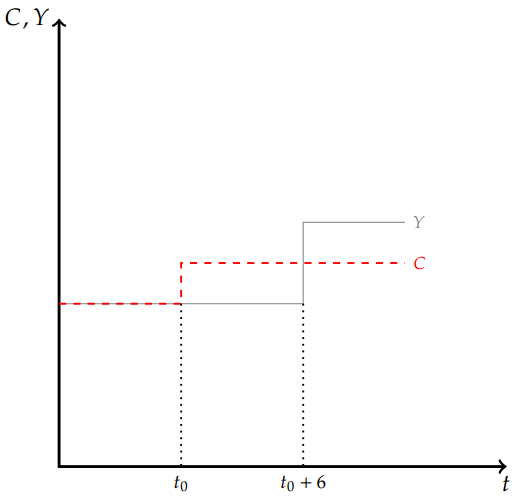
\includegraphics[scale=0.7]{../Figures/C35.3.png} 
    \end{center} 
\end{frame}

\begin{frame}{Modelo de elección del consumo presente y consumo futuro: restricción intertemporal SIN crédito}
    \begin{center}
        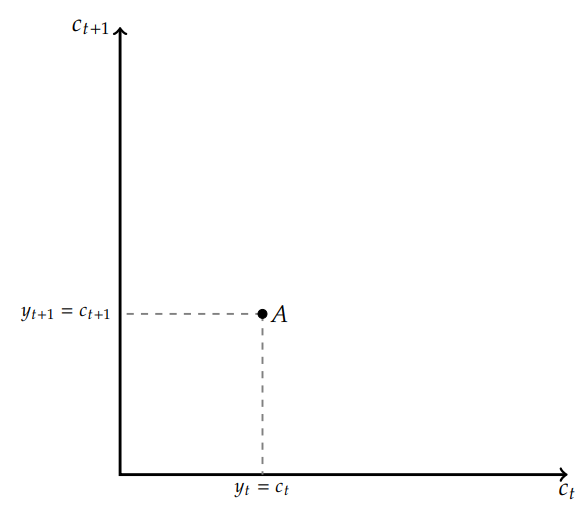
\includegraphics[scale=0.7]{../Figures/C35.4.png} 
    \end{center} 
\end{frame}

\begin{frame}{Modelo de elección del consumo presente y consumo futuro: restricción intertemporal CON crédito}
    Si hay crédito, puedo armar una restricción presupuestaria jugando con la tasa de interés.

    Partiendo de la siguiente igualdad:

    \[y_t = c_t + a_t\]
    donde \(y_t\) es el ingreso, \(c_t\) es el consumo y \(a_t\) es el ahorro del período, en el período siguiente se podrá consumir el ingreso de ese período, más lo que se ahorro el período anterior multiplicado por la tasa de interés (simplifiquemos pensando que en $t+1$ se consume todo y no se ahorra):

    \[c_{t+1} = y_{t+1} + (1+r)\,a_t\]
    Si reemplazo $a_t$ de la primera ecuación en la segunda, obtengo:
    \[c_{t+1} = y_{t+1} + (1+r)\,(y_t - c_t)\]
\end{frame}

\begin{frame}{Modelo de elección del consumo presente y consumo futuro: restricción intertemporal CON crédito}
    Donde luego
    \[c_{t+1} = y_{t+1} + (1+r)\,y_t - (1+r)\,c_t\]
    Donde queda formada una restricción presupuestaria entre el consumo presente y el consumo futuro. Características:
    \begin{itemize}
        \item Pendiente $-(1+r)$: Si consumo una unidad menos hoy, consumo $(1+r)$ más mañana. Si consumo una unidad más hoy, consumo $-(1+r)$ mañana.
        \item Ordenada al origen $c_{t+1} = y_{t+1} + (1+r)\,y_t$: Si no consumo nada hoy, consumo $y_{t+1} + (1+r)\,y_t$ mañana. Ahorré todo!
        \item Raíz $c_t = y_t + y_{t+1}/(1+r)$: Si consumo todo hoy, consumo $y_t + y_{t+1}/(1+r)$ mañana. Pedí prestado todo lo que iba a tener de ingreso el período siguiente!
    \end{itemize}
\end{frame}

\begin{frame}{Modelo de elección del consumo presente y consumo futuro: restricción intertemporal CON crédito}
    \begin{center}
        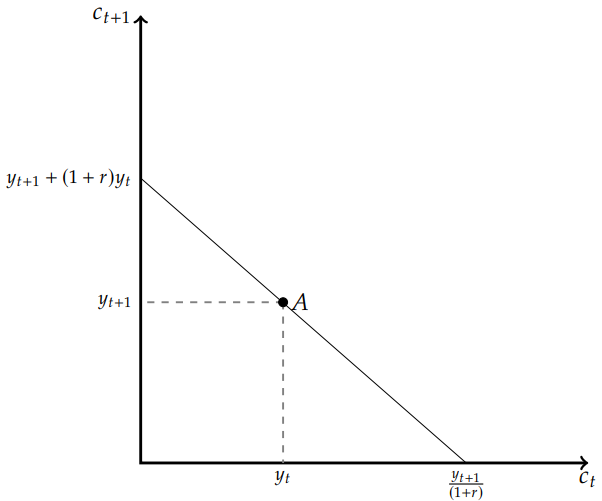
\includegraphics[scale=0.65]{../Figures/C35.5.png}
    \end{center} 
\end{frame}


\begin{frame}{Modelo de elección del consumo presente y consumo futuro: la curva de indiferencia}
    \begin{center}
        \begin{figure}[H]
        \renewcommand{\figurename}{Figure}
            \begin{center}
                \begin{tikzpicture}[scale=0.6]
                \draw[very thick,<->] (0,11) node[left]{$c_{t+1}$}--(0,0)--(11,0) node[below]{$c_{t}$};
                \draw[semithick] (2,8).. controls (2.5,2.5) and (4,0.75) ..(8.25,0.65);
                \draw[thick, gray, dashed](2.15, 7)--(2.85, 4);
                \draw[fill] (2.1,7) circle [radius =0.11] ;
                \draw[thick, gray, dashed](4.2, 1.9)--(2.85, 4);      
                \draw[fill] (2.8,3.95) circle [radius =0.11] ;
                \draw[fill] (4.2,1.8) circle [radius =0.11] ;      
                \draw[semithick, ->] (2.1,7)--(2.1,4);
                \draw[semithick, ->] (2.1,3.95)--(2.7,3.95);
                \draw[semithick, ->] (2.8,3.95)--(2.8,1.8);
                \draw[semithick, ->] (2.85,1.8)--(4,1.8);
                \end{tikzpicture}
            \end{center}
        \end{figure}
    \end{center}
\end{frame}

\begin{frame}{Modelo de elección del consumo presente y consumo futuro: el equilibrio}
    \begin{center}
        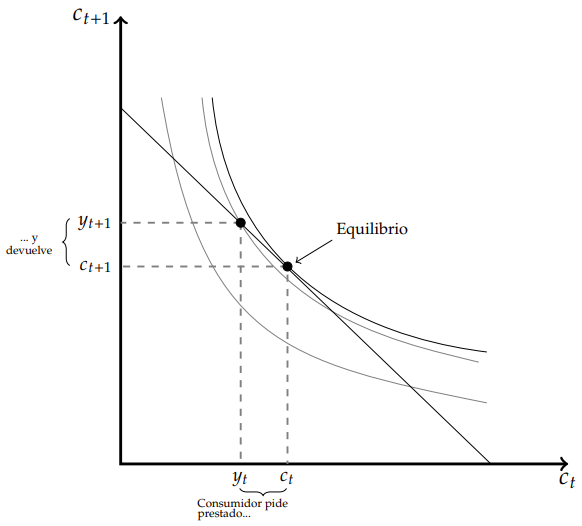
\includegraphics[scale=0.65]{../Figures/C35.6.png}
    \end{center}  
\end{frame}

\begin{frame}{El efecto de un cambio en la tasa de interés}
    \begin{itemize}
        \item La tasa de interés no es otra cosa que el precio del consumo presente relativo al consumo futuro, entonces el cambio en la tasa de interés se puede descomponer en un efecto ingreso y un efecto sustitución.
        \begin{itemize}
            \item \textbf{ES}: lleva a consumir menos (ahorrar más) ante aumentos en la tasa de interés. Se vuelve más atractivo ahorrar porque aumenta el costo de oportunidad de consumir en el presente.
            \item \textbf{EI}: que me vuelva más rico o no depende de mi situación inicial:
            \begin{itemize}
                \item Si soy un ahorrista neto, me vuelvo más rico porque el valor presente de mis ahorros aumenta.
                \item Si soy un deudor neto, me vuelvo más pobre porque el valor presente de mis deudas aumenta.
            \end{itemize}
            \item En general, el efecto sustitución es más fuerte que el efecto ingreso porque el efecto ingreso se compensa entre deudores y acreedores.
        \end{itemize}
        \item Por eso, ante aumentos en la tasa de interes estos modelos muestran que aumenta el ahorro (baja el consumo) y visceversa ante caidas en la tasa de interes.
    \end{itemize}
\end{frame}


\begin{frame}{El efecto de un cambio en la tasa de interés}
    \begin{center}
        \begin{figure}[H]
        \renewcommand{\figurename}{Figure}
            \begin{center}
                \begin{tikzpicture}[scale=0.45]
                    \draw[very thick,<->] (0,15) node[left]{$c_{t+1}$}--(0,0)--(15,0) node[below]{$c_{t}$}; % ejes
                    \draw[semithick] (2.25,9).. controls (2.75,4) and (7, 3) .. (9, 2.75); % CI 1
                    \draw[semithick] (0,8.75)--(9.1,0); % Restricción presupuestaria 1
                    \draw[semithick, blue] (0,7.4)--(11.6,0); % Recta con mayor interés
                    \draw[thick, gray, dashed](4.1, 4.65)--(4.1, 0);
                    \draw[thick, gray, dashed](4.1, 4.85)--(0, 4.85);
                    \draw[fill] (4.1,4.85) circle [radius =0.11] ;  
                    \node[below] at (4,0) {\footnotesize $y_t = c_t$};
                    \node[left] at (0,4.85){\footnotesize $y_{t+1} = c_{t+1}$};
                \end{tikzpicture}
            \end{center}
        \end{figure}
    \end{center}  
\end{frame}

\begin{frame}{Otras teorías del ahorro}
   \begin{itemize}
       \item Ciclo de vida
       \item Hipotecas revertidas
       \item Los tests de Shea
       \item Ahorro precautorio
       \item La fuerza de los defaults
       \item Present bias
   \end{itemize} 
\end{frame}


\begin{frame}{La inversión: valor presente}
    La inversión se decide en base al valor presente de los flujos futuros de ingreso que genera un determinado proyecto.
    \begin{equation}
        VPN = I_0 + \sum_{t=1} ^{T} \frac{1}{(1+r)^t} R_t,
    \end{equation}
    \begin{itemize}
        \item $r$ es el costo del capital.
        \item $I_0$ es el costo inicial.
        \item ¿Cuanta plata necesito hoy para tener $R_t$ en el futuro? Como entre ahora y $t$, cualquier dinero podemos ponerlo a rendir un interés del mercado, el equivalente hoy de un dinero futuro será menor.
        \item Si el VPN$>0$, entonces convendría invertir.
        \item Si VPN $<0$ no convendría.
        \item ¿Tarjetas de crédito? ¿Inflación?
    \end{itemize}
\end{frame}

\begin{frame}{Demanda agregada y el mercado de crédito}

$$ Y = C(r) + I(r) + G $$

\centering \small{donde r es la tasa de interés real}

\begin{itemize}
\item En una economía cerrada:
$$ Y – C(r) – G = I(r) $$
\end{itemize}
\begin{itemize}
\item Que es como decir que lo que ahorro es lo que invierto
\item Y esto determina la tasa de interés real
\item Los ahorros son intermediados por el sector financiero hacia inversiones reales
\item Economías que ahorran mucho invierten mucho (China, Japón), economías que ahorran poco invierten menos (Brasil, Argentina)! 
\end{itemize}
\end{frame}


\begin{frame}{El mercado de crédito}
    \begin{center}
        \begin{figure}[H]
        \renewcommand{\figurename}{Figure}
            \begin{center}
                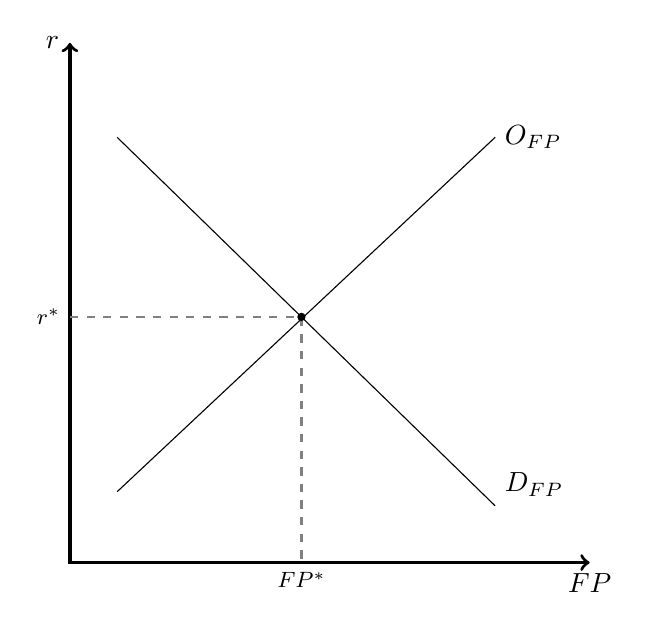
\begin{tikzpicture}[scale=0.6]
                    \draw[very thick,<->] (0,11) node[left]{$r$}--(0,0)--(11,0) node[below]{$FP$};
                    \draw[thin](1,1.5)--(9,9) node [right] {$O_{FP}$};
                    \draw[thin](1,9)--(9,1.2) node [above right] {$D_{FP}$};
                    \draw[thick,dashed,gray] (0,5.2)--(4.9,5.2)--(4.9,0);
                    \draw[fill] (4.9,5.2) circle [radius =0.075]; 
                    \node[below] at (4.9,0) {\footnotesize $FP^{*}$};
                    \node[left] at (0,5.2) {\footnotesize $r^{*}$};
                \end{tikzpicture}
            \end{center}
        \end{figure}
    \end{center}  
\end{frame}

\begin{frame}{El mercado de crédito}
    \begin{itemize}
        \item La tasa de interés de equilibrio se alcanza cuando la demanda de crédito (demanda de fondos prestables) se iguala con la oferta de crédito (oferta de fondos prestables).
        \item Un aumento en la inversión desplaza la curva de crédito hacia arriba (se demandan más prestamos), lo que aumenta la tasa de interés.
        \item En el mismo sentido:
        \begin{itemize}
            \item Un aumento en la deuda del gobierno (financia deficit con deuda).
        \end{itemize}
        \item Como en estos dos ultimos casos aumenta la tasa de interes, eso hará caer la inversión (en equilibrio), que es lo que llamamos \textit{crowding out}.
        \item Un aumento en el ahorro desplaza la curva de oferta de fondos prestables hacia abajo, permitiendo una menor tasa de interés de equilibrio.
    \end{itemize}
    
\end{frame}

\begin{frame}{El mercado de crédito}
    \begin{center}
        \begin{figure}[H]
        \renewcommand{\figurename}{Figure}
            \begin{center}
                    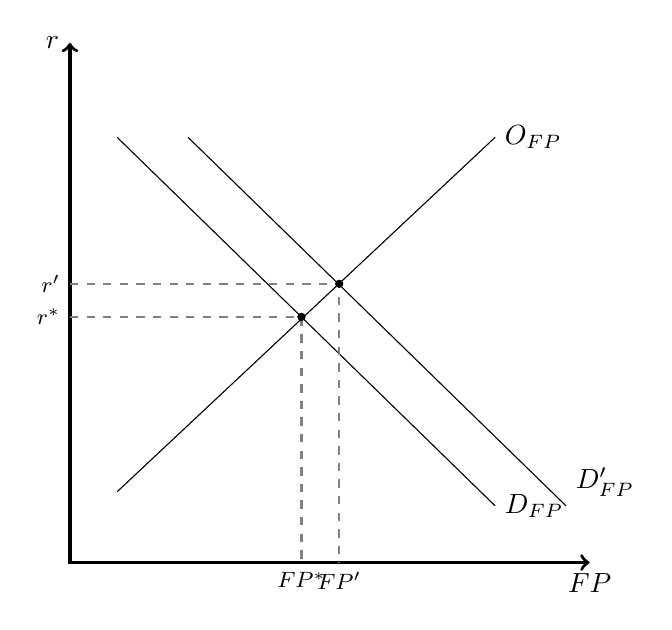
\begin{tikzpicture}[scale=0.6]
                        \draw[very thick,<->] (0,11) node[left]{$r$}--(0,0)--(11,0) node[below]{$FP$};
                        \draw[thin](1,1.5)--(9,9) node [right] {$O_{FP}$};
                        \draw[thin](1,9)--(9,1.2) node [right] {$D_{FP}$};
                        \draw[thin](2.5,9)--(10.5,1.2) node [above right] {$D_{FP}'$};
                        \draw[thick,dashed,gray] (0,5.2)--(4.9,5.2)--(4.9,0);
                        \draw[thick,dashed,gray] (0,5.9)--(5.7,5.9)--(5.7,0);
                        \draw[fill] (4.9,5.2) circle [radius =0.075]; 
                        \draw[fill] (5.7,5.9) circle [radius =0.075]; 
                        \node[below] at (4.9,0) {\footnotesize $FP^{*}$};
                        \node[left] at (0,5.2) {\footnotesize $r^{*}$};
                        \node[below] at (5.7,0) {\footnotesize $FP'$};
                        \node[left] at (0,5.9) {\footnotesize $r'$};
                    \end{tikzpicture}
            \end{center}
        \end{figure}
    \end{center}  
\end{frame}



\end{document}